% Created by tikzDevice version 0.12.3 on 2020-12-17 11:19:17
% !TEX encoding = UTF-8 Unicode
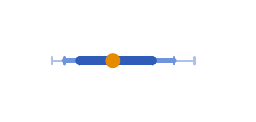
\begin{tikzpicture}[x=1pt,y=1pt]
\definecolor{fillColor}{RGB}{255,255,255}
\path[use as bounding box,fill=fillColor,fill opacity=0.00] (0,0) rectangle ( 72.27, 23.85);
\begin{scope}
\path[clip] (  0.00,  0.00) rectangle ( 72.27, 23.85);
\definecolor{drawColor}{RGB}{173,194,235}

\path[draw=drawColor,line width= 0.8pt,line join=round,line cap=round] (  8.74, 11.92) --
	( 60.29, 11.92);

\path[draw=drawColor,line width= 0.8pt,line join=round,line cap=round] (  8.74, 10.60) --
	(  8.74, 13.25);

\path[draw=drawColor,line width= 0.8pt,line join=round,line cap=round] ( 60.29, 10.60) --
	( 60.29, 13.25);
\definecolor{drawColor}{RGB}{112,148,219}

\path[draw=drawColor,line width= 2.0pt,line join=round,line cap=round] ( 13.31, 11.92) --
	( 52.85, 11.92);

\path[draw=drawColor,line width= 0.8pt,line join=round,line cap=round] ( 13.31, 10.60) --
	( 13.31, 13.25);

\path[draw=drawColor,line width= 0.8pt,line join=round,line cap=round] ( 52.85, 10.60) --
	( 52.85, 13.25);
\definecolor{drawColor}{RGB}{46,92,184}

\path[draw=drawColor,line width= 3.2pt,line join=round,line cap=round] ( 18.76, 11.92) --
	( 45.12, 11.92);

\path[draw=drawColor,line width= 0.8pt,line join=round,line cap=round] ( 18.76, 10.60) --
	( 18.76, 13.25);

\path[draw=drawColor,line width= 0.8pt,line join=round,line cap=round] ( 45.12, 10.60) --
	( 45.12, 13.25);
\definecolor{fillColor}{RGB}{230,138,0}

\path[fill=fillColor] ( 30.78, 11.92) circle (  2.70);
\end{scope}
\end{tikzpicture}
